\documentclass[letter,12pt]{article}
\usepackage[paperheight=27.94cm,paperwidth=21.59cm,bindingoffset=0in,left=3cm,right=2.0cm, top=3.5cm,bottom=2.5cm, headheight=200pt, headsep=1.0\baselineskip]{geometry}
\usepackage{graphicx,lastpage}
\usepackage{upgreek}
\usepackage{censor}
\usepackage[spanish,es-tabla]{babel}
\usepackage{pdfpages}
\usepackage{tabularx}
\usepackage{graphicx}
\usepackage{adjustbox}
\usepackage{xcolor}
\usepackage{colortbl}
\usepackage{rotating}
\usepackage{multirow}
\usepackage[utf8]{inputenc}
\usepackage{float}
\usepackage{hyperref}

\renewcommand{\tablename}{Tabla}
\usepackage{fancyhdr}
\pagestyle{fancy}

\usepackage{listing}
\usepackage{lstautogobble}
\newcommand{\code}[1]{\colorbox{lightgray!80}{\lstinline[breaklines=true]|#1|}}
\newcommand{\BashCode}{
    \lstset{
        language=bash,
        basicstyle=\ttfamily\small,
        backgroundcolor=\color{lightgray!30},
        breaklines=true,
        showspaces=false,
        showstringspaces=false,
        numbers=left,
        % listings no tiene definido utf-8 por defecto
        % definimos cada carácter especial
        literate=
          {á}{{\'a}}1
          {é}{{\'e}}1
          {í}{{\'\i}}1
          {ó}{{\'o}}1
          {ú}{{\'u}}1
          {ñ}{{\~n}}1
          {¡}{{!`}}1
          {¿}{{?`}}1
      }
}

\begin{document}
   \title{\Huge{Informe Laboratorio 4}}
   \author{\textbf{Sección 3} \\  \\Alan Toro \\ e-mail: alan.toro@mail.udp.cl}
   \date{Noviembre de 2023}
   \maketitle
   \tableofcontents
  \newpage

\section{Descripción de actividades}
Para este laboratorio, deberá utilizar Tampermonkey y la librería CryptoJS (con
SRI) para lograr obtener los mensajes que le está comunicando su informante. En
esta ocasión, su informante fue más osado y se comunicó con usted a través de un
sitio web abierto a todo el público https://cripto.tiiny.site/.\par Sólo un ojo
entrenado como el suyo logrará descifrar cuál es el algoritmo de cifrado
utilizado y cuál es la contraseña utilizada para lograr obtener la información
que está oculta.
\begin{enumerate}
    \item Desarrolle un plugin para tampermonkey que permita obtener la llave
      para el descifrado de los mensajes ocultos en la página web. La llave debe
      ser impresa por la consola de su navegador al momento de cargar el sitio
      web. Utilizar la siguiente estructura:
    \begin{itemize}
        \item   La llave es: KEY
    \end{itemize}
    \item En el mismo plugin, se debe detectar el patrón que permite identificar
      la cantidad de mensajes cifrados. Debe imprimir por la consola la cantidad
      de mensajes cifrados. Utilizar la siguiente estructura: Los mensajes
      cifrados son: NUMBER
    \item En el mismo plugin debe obtener cada mensaje cifrado y descifrarlo.
      Ambos mensajes deben ser informados por la consola (cifrado espacio
      descifrado) y además cada mensaje en texto plano debe ser impreso en la
      página web. \par El script desarrollado debe ser capaz de obtener toda la
      información del sitio web (llave, cantidad de mensajes, mensajes cifrados)
      sin ningún valor forzado. Para verificar el correcto funcionamiento de su
      script se utilizará un sitio web con otro texto y una cantidad distinta de
      mensajes cifrados. Deberá indicar la url donde se podrá descargar su
      script.\par Un ejemplo de lo que se debe visualizar en la consola, al
      ejecutar automáticamente el script, es lo siguiente:
    \begin{figure}[H]
        \centering 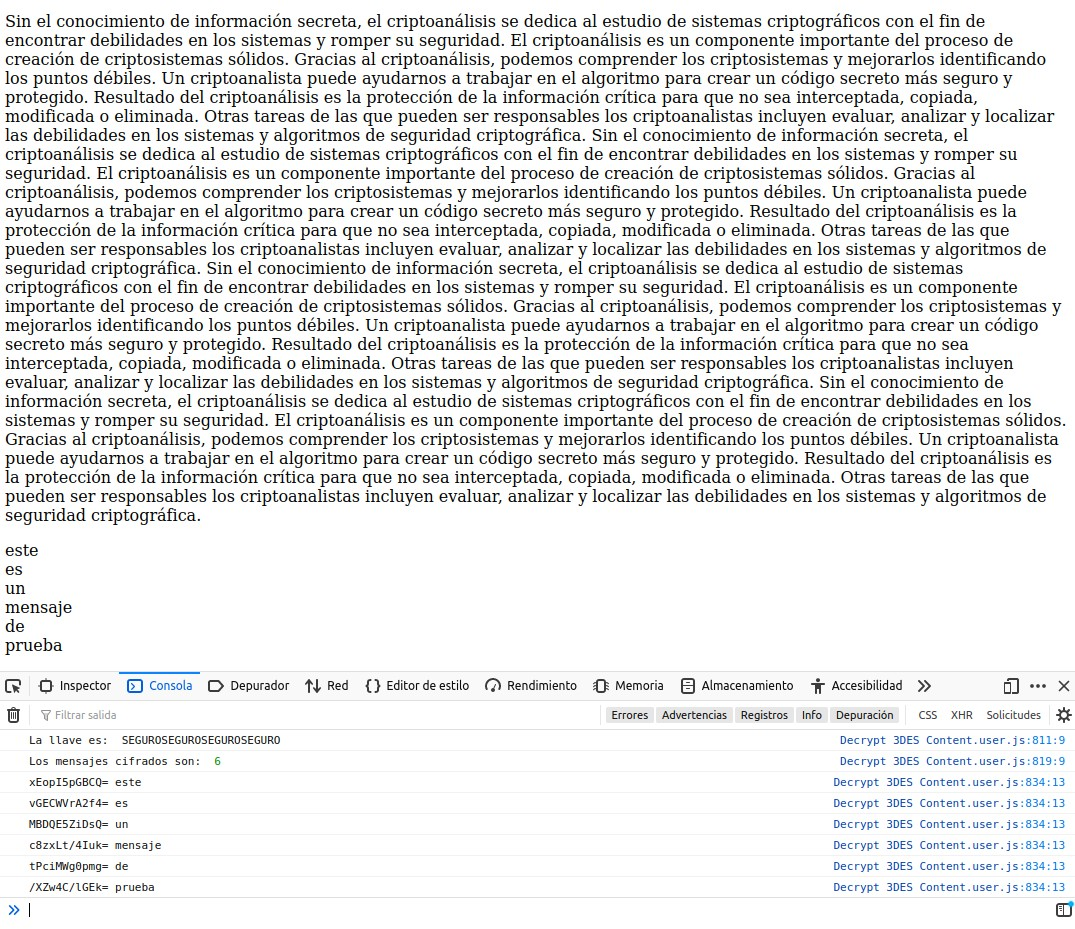
\includegraphics[width=16cm]{Desarrollo/ejemplo.png}
        \label{fig:ejemplo}
    \end{figure}
\end{enumerate}

\section{Desarrollo (Parte 1)}
\subsection{Detecta el cifrado utilizado por el informante}
Se conoce de antemano la llave como ``SEGUROSEGUROSEGUROSEGURO'', Por inspección
simple se puede notar que las letras son todas mayúsculas y que además, son las
únicas mayúsculas dentro del documento.
\subsection{Logra que el script solo se gatille en el sitio usado por el informante}
Para gatillar el script se puede usar la directiva \code{@match} con la URL a la
cuál se espera usar para gatillar el script.


\begin{listing}
    \BashCode{}
  \begin{lstlisting}
@match        https://cripto.tiiny.site/
  \end{lstlisting}
\end{listing}

\subsection{Define función que obtiene automáticamente el password del documento}
Para buscar el mensaje dentro del texto, primero se selecciona la etiqueta "p",
se aplica una expresión regular buscando letras mayúsculas lo que retorna un
arreglo de los caractéres en mayúsculas que se encuentran y se le aplica join()
para transformar de array a string.

\begin{listing}
    \BashCode{}
  \begin{lstlisting}
let key = document.querySelector('p').textContent.match(/[A-Z]/g).join("")
console.log("La llave es: ", key)
  \end{lstlisting}
\end{listing}

\subsection{Muestra la llave por consola}
Al ejecutarse el script muestra por consola la llave encontrada con el formato ``La llave es: KEY''.

\begin{figure}[H]
  \centering
  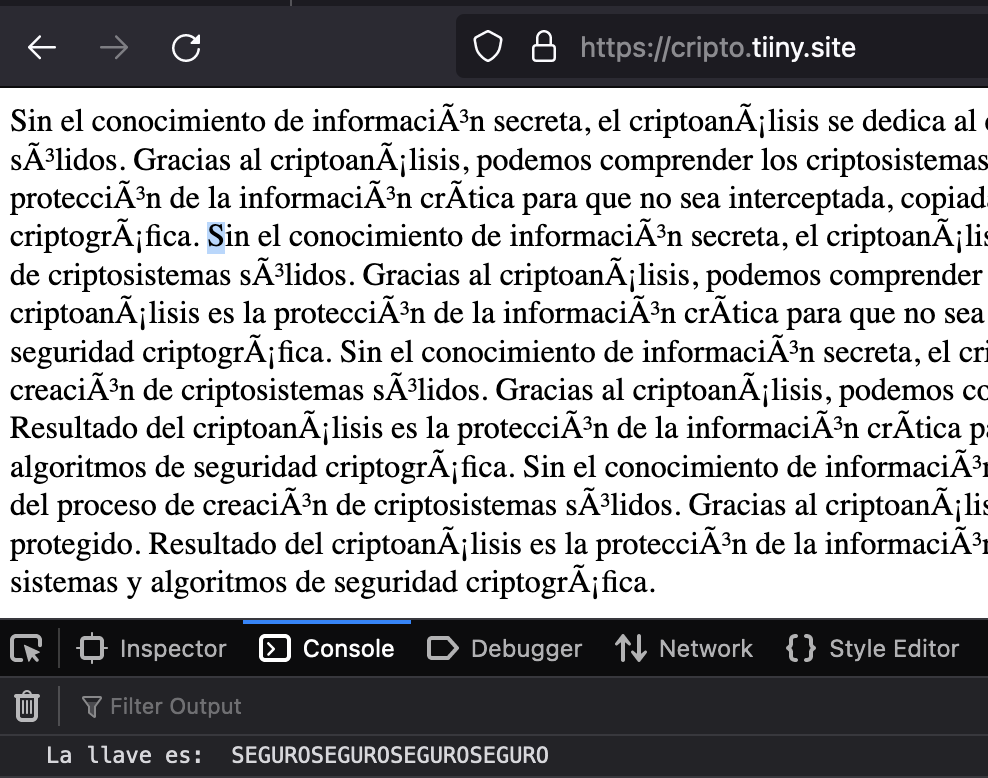
\includegraphics[width=16cm]{images/01-key-console.png}
  \caption{Ejecución del script y llave mostrada en consola.}
\end{figure}

\section{Desarrollo (Parte 2)}
\subsection{Reconoce automáticamente la cantidad de mensajes cifrados}
Además de la etiqueta "p" se encuentran etiquetas "div" sin contenido en donde
el id terminar en ``='' por lo que se puede intuir que son mensajes en base64.
Se genera entonces un script que cuente las etiquetas "div" en el documento.

\begin{listing}
    \BashCode{}
  \begin{lstlisting}
let msgs = document.querySelectorAll('div')
console.log("Los mensajes cifrados son: ", msgs.length)
  \end{lstlisting}
\end{listing}

\subsection{Muestra la cantidad de mensajes por consola}
Se muestran entonces la cantidad de mensajes cifrados dentro de la página.

\begin{figure}[H]
  \centering
  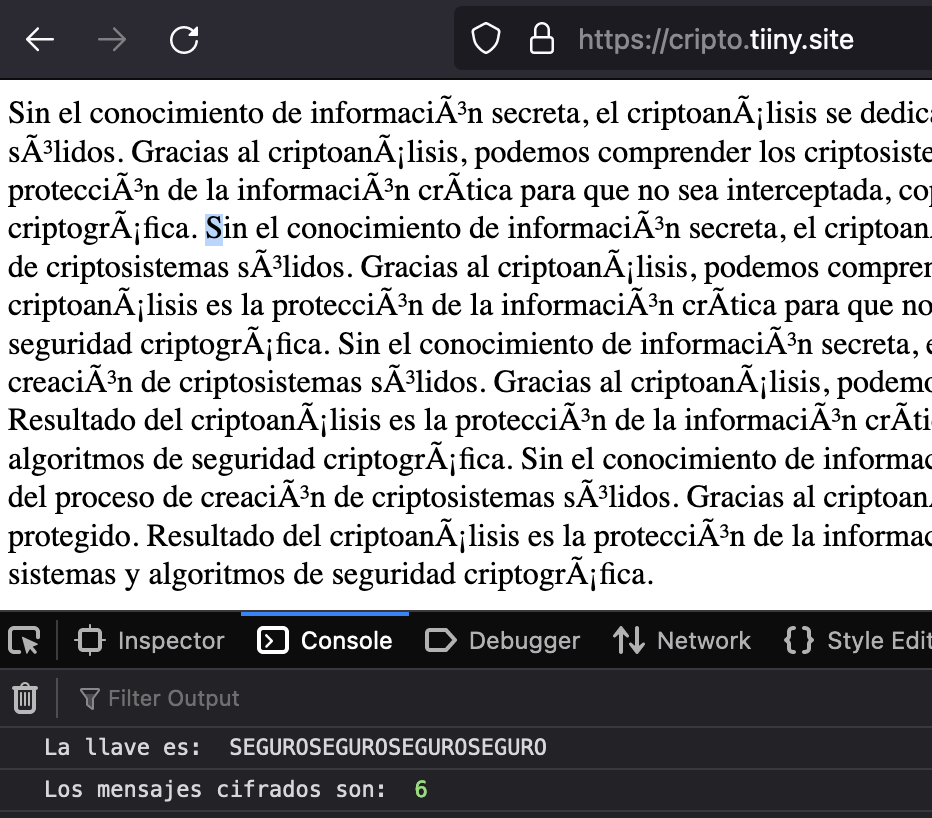
\includegraphics[width=13cm]{images/02-cant-msg.png}
  \caption{Cantidad de mensajes cifrados.}
\end{figure}

\section{Desarrollo (Parte 3)}

\subsection{Importa la librería cryptoJS}
Para importar librerías con Tampermonkey se utiliza la directiva
\code{@require}, con esta basta con entregarle la URL de la librería para tener
disponible la librería.

\subsection{Utiliza SRI en la librería CryptoJS}
Además, la directiva \code{@require} permite de forma nativa utilizar una url en
el formato url\#hash para el SRI, en donde el hash puede estar en MD5 o
SHA-512 (que es el utilizado para la revisión de integridad en cdnjs que es el
utilizado en este informe).

Para visualizar el uso de la directiva se puede ver en el script adjunto a este
trabajo.

\subsection{Logra decifrar uno de los mensajes}
De la imagen entregada en el enunciado se sabe que el método para decifrar debe
ser 3DES.  Para esto, la librería CryptoJS exige recibir el texto encriptado y
la llave ambos en base64, además de definir el método de padding y el modo.

El mensaje cifrado ya se encuentra en base64 por lo que basta con parsearlo.
Para la llave (que se encuentra en texto plano) es necesario transformarla a base64 utilizando

\begin{listing}
    \BashCode{}
  \begin{lstlisting}
let keyBase64 = CryptoJS.enc.Base64.stringify(CryptoJS.enc.Utf8.parse(key))
  \end{lstlisting}
\end{listing}

Para luego parsearla de la misma manera que el mensaje. Esto se realiza usando

\begin{listing}
    \BashCode{}
  \begin{lstlisting}
CryptoJS.enc.Base64.parse(<textToParse>)
  \end{lstlisting}
\end{listing}

Con lo anterior se puede decifrar el mensaje usando:

\begin{listing}
    \BashCode{}
  \begin{lstlisting}
CryptoJS.TripleDES.decrypt(msg.id, parsedKey, {mode: CryptoJS.mode.ECB, padding: CryptoJS.pad.Pkcs7})
  \end{lstlisting}
\end{listing}

\subsection{Imprime todos los mensajes por consola}
Se repite el proceso por cada uno de los mensajes guardados por cada uno de los mensajes cifrados.

\begin{figure}[H]
  \centering
  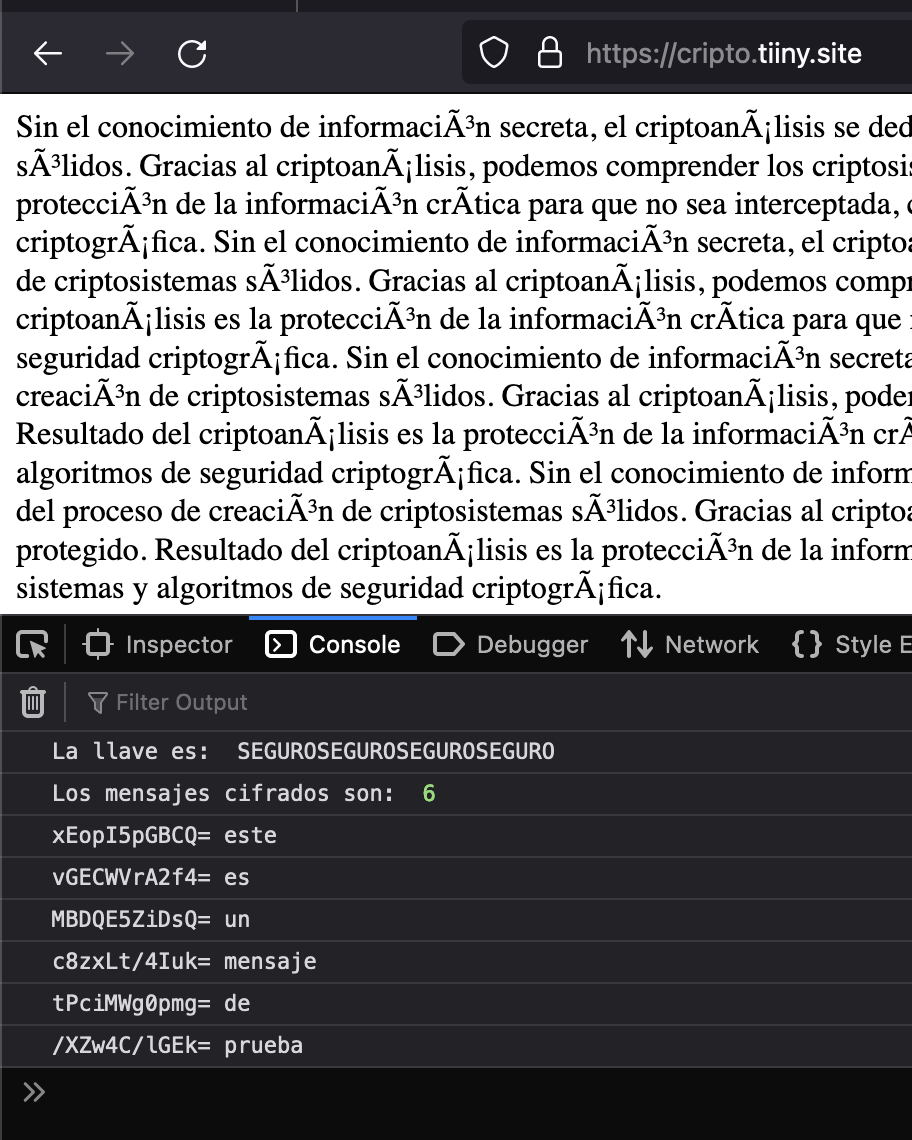
\includegraphics[width=13cm]{images/03-all-msgs.png}
  \caption{Mensajes mostrados en la consola en texto plano.}
\end{figure}

\subsection{Muestra los mensajes en texto plano en el sitio web}
Finalmente, los mensajes cifrados además de mostrarse en consola se agregan a la etiqueta "p" cada uno de los mensajes decifrados en texto plano.

\begin{figure}[H]
  \centering
  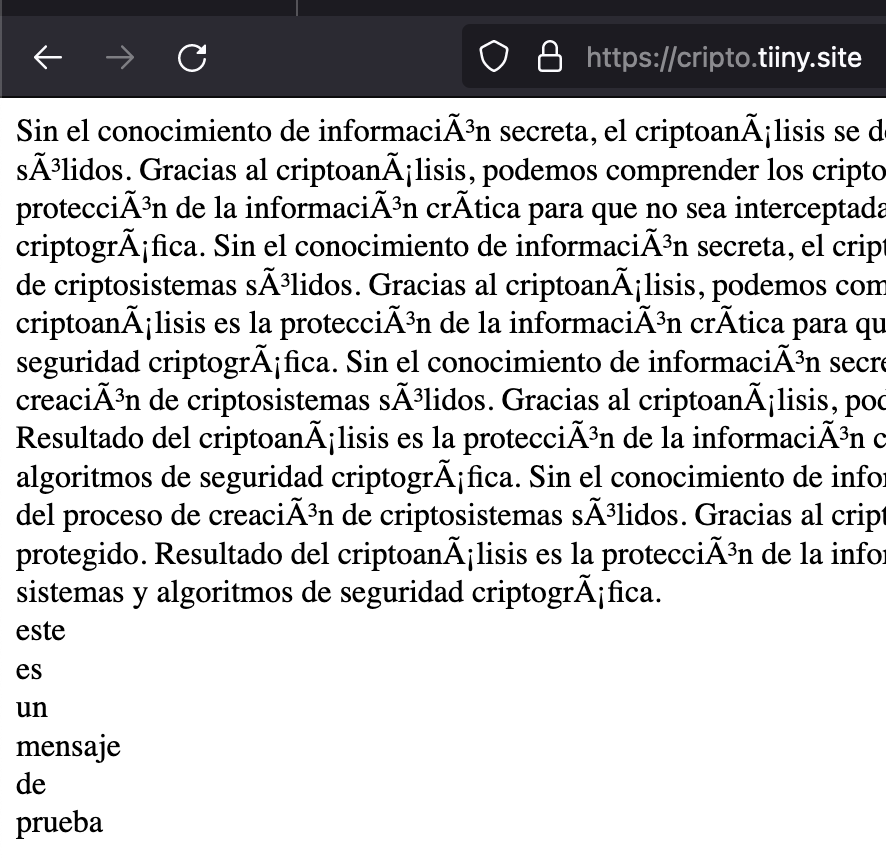
\includegraphics[width=13cm]{images/04-msgs.png}
  \caption{Mensajes mostrados en la consola en texto plano.}
\end{figure}

\subsection{El script logra funcionar con otro texto y otra cantidad de mensajes}
Las invariantes que considera el script son que el texto tenga una llave escondida entre las mayúsculas y la cantidad de mensajes son tantos como etiquetas div existan.

\subsection{Indica url al código .js implementado para su validación}
El archivo lab4/Lab4.js del repositorio \url{https://github.com/wzrdd/cripto} contiene el script utilizado.

\section*{Conclusiones y comentarios}
En la pasada experiencia se puede mostrar una manera de transmitir un mensaje dentro de un medio público con un poco de ingenio (usar las mayúsculas de un texto) y la utilización de métodos de cifrado para ofuscar o dificultar su decifrado.

\end{document}
